% Options for packages loaded elsewhere
\PassOptionsToPackage{unicode}{hyperref}
\PassOptionsToPackage{hyphens}{url}
%
\documentclass[
  paper=6in:9in,
  pagesize=pdftex,
  headinclude=on,
  footinclude=on,
  12pt]{scrbook}

\usepackage{amsmath,amssymb}
\usepackage{iftex}
\ifPDFTeX
  \usepackage[T1]{fontenc}
  \usepackage[utf8]{inputenc}
  \usepackage{textcomp} % provide euro and other symbols
\else % if luatex or xetex
  \usepackage{unicode-math}
  \defaultfontfeatures{Scale=MatchLowercase}
  \defaultfontfeatures[\rmfamily]{Ligatures=TeX,Scale=1}
\fi
\usepackage{lmodern}
\ifPDFTeX\else  
    % xetex/luatex font selection
\fi
% Use upquote if available, for straight quotes in verbatim environments
\IfFileExists{upquote.sty}{\usepackage{upquote}}{}
\IfFileExists{microtype.sty}{% use microtype if available
  \usepackage[]{microtype}
  \UseMicrotypeSet[protrusion]{basicmath} % disable protrusion for tt fonts
}{}
\makeatletter
\@ifundefined{KOMAClassName}{% if non-KOMA class
  \IfFileExists{parskip.sty}{%
    \usepackage{parskip}
  }{% else
    \setlength{\parindent}{0pt}
    \setlength{\parskip}{6pt plus 2pt minus 1pt}}
}{% if KOMA class
  \KOMAoptions{parskip=half}}
\makeatother
\usepackage{xcolor}
\setlength{\emergencystretch}{3em} % prevent overfull lines
\setcounter{secnumdepth}{5}
% Make \paragraph and \subparagraph free-standing
\ifx\paragraph\undefined\else
  \let\oldparagraph\paragraph
  \renewcommand{\paragraph}[1]{\oldparagraph{#1}\mbox{}}
\fi
\ifx\subparagraph\undefined\else
  \let\oldsubparagraph\subparagraph
  \renewcommand{\subparagraph}[1]{\oldsubparagraph{#1}\mbox{}}
\fi


\providecommand{\tightlist}{%
  \setlength{\itemsep}{0pt}\setlength{\parskip}{0pt}}\usepackage{longtable,booktabs,array}
\usepackage{calc} % for calculating minipage widths
% Correct order of tables after \paragraph or \subparagraph
\usepackage{etoolbox}
\makeatletter
\patchcmd\longtable{\par}{\if@noskipsec\mbox{}\fi\par}{}{}
\makeatother
% Allow footnotes in longtable head/foot
\IfFileExists{footnotehyper.sty}{\usepackage{footnotehyper}}{\usepackage{footnote}}
\makesavenoteenv{longtable}
\usepackage{graphicx}
\makeatletter
\def\maxwidth{\ifdim\Gin@nat@width>\linewidth\linewidth\else\Gin@nat@width\fi}
\def\maxheight{\ifdim\Gin@nat@height>\textheight\textheight\else\Gin@nat@height\fi}
\makeatother
% Scale images if necessary, so that they will not overflow the page
% margins by default, and it is still possible to overwrite the defaults
% using explicit options in \includegraphics[width, height, ...]{}
\setkeys{Gin}{width=\maxwidth,height=\maxheight,keepaspectratio}
% Set default figure placement to htbp
\makeatletter
\def\fps@figure{htbp}
\makeatother
% definitions for citeproc citations
\NewDocumentCommand\citeproctext{}{}
\NewDocumentCommand\citeproc{mm}{%
  \begingroup\def\citeproctext{#2}\cite{#1}\endgroup}
\makeatletter
 % allow citations to break across lines
 \let\@cite@ofmt\@firstofone
 % avoid brackets around text for \cite:
 \def\@biblabel#1{}
 \def\@cite#1#2{{#1\if@tempswa , #2\fi}}
\makeatother
\newlength{\cslhangindent}
\setlength{\cslhangindent}{1.5em}
\newlength{\csllabelwidth}
\setlength{\csllabelwidth}{3em}
\newenvironment{CSLReferences}[2] % #1 hanging-indent, #2 entry-spacing
 {\begin{list}{}{%
  \setlength{\itemindent}{0pt}
  \setlength{\leftmargin}{0pt}
  \setlength{\parsep}{0pt}
  % turn on hanging indent if param 1 is 1
  \ifodd #1
   \setlength{\leftmargin}{\cslhangindent}
   \setlength{\itemindent}{-1\cslhangindent}
  \fi
  % set entry spacing
  \setlength{\itemsep}{#2\baselineskip}}}
 {\end{list}}
\usepackage{calc}
\newcommand{\CSLBlock}[1]{\hfill\break\parbox[t]{\linewidth}{\strut\ignorespaces#1\strut}}
\newcommand{\CSLLeftMargin}[1]{\parbox[t]{\csllabelwidth}{\strut#1\strut}}
\newcommand{\CSLRightInline}[1]{\parbox[t]{\linewidth - \csllabelwidth}{\strut#1\strut}}
\newcommand{\CSLIndent}[1]{\hspace{\cslhangindent}#1}

\usepackage{fvextra}
\DefineVerbatimEnvironment{Highlighting}{Verbatim}{breaklines,commandchars=\\\{\}}
\areaset[0.50in]{4.5in}{8in}
\makeatletter
\@ifpackageloaded{tcolorbox}{}{\usepackage[skins,breakable]{tcolorbox}}
\@ifpackageloaded{fontawesome5}{}{\usepackage{fontawesome5}}
\definecolor{quarto-callout-color}{HTML}{909090}
\definecolor{quarto-callout-note-color}{HTML}{0758E5}
\definecolor{quarto-callout-important-color}{HTML}{CC1914}
\definecolor{quarto-callout-warning-color}{HTML}{EB9113}
\definecolor{quarto-callout-tip-color}{HTML}{00A047}
\definecolor{quarto-callout-caution-color}{HTML}{FC5300}
\definecolor{quarto-callout-color-frame}{HTML}{acacac}
\definecolor{quarto-callout-note-color-frame}{HTML}{4582ec}
\definecolor{quarto-callout-important-color-frame}{HTML}{d9534f}
\definecolor{quarto-callout-warning-color-frame}{HTML}{f0ad4e}
\definecolor{quarto-callout-tip-color-frame}{HTML}{02b875}
\definecolor{quarto-callout-caution-color-frame}{HTML}{fd7e14}
\makeatother
\makeatletter
\@ifpackageloaded{caption}{}{\usepackage{caption}}
\AtBeginDocument{%
\ifdefined\contentsname
  \renewcommand*\contentsname{Table of contents}
\else
  \newcommand\contentsname{Table of contents}
\fi
\ifdefined\listfigurename
  \renewcommand*\listfigurename{List of Figures}
\else
  \newcommand\listfigurename{List of Figures}
\fi
\ifdefined\listtablename
  \renewcommand*\listtablename{List of Tables}
\else
  \newcommand\listtablename{List of Tables}
\fi
\ifdefined\figurename
  \renewcommand*\figurename{Figure}
\else
  \newcommand\figurename{Figure}
\fi
\ifdefined\tablename
  \renewcommand*\tablename{Table}
\else
  \newcommand\tablename{Table}
\fi
}
\@ifpackageloaded{float}{}{\usepackage{float}}
\floatstyle{ruled}
\@ifundefined{c@chapter}{\newfloat{codelisting}{h}{lop}}{\newfloat{codelisting}{h}{lop}[chapter]}
\floatname{codelisting}{Listing}
\newcommand*\listoflistings{\listof{codelisting}{List of Listings}}
\makeatother
\makeatletter
\makeatother
\makeatletter
\@ifpackageloaded{caption}{}{\usepackage{caption}}
\@ifpackageloaded{subcaption}{}{\usepackage{subcaption}}
\makeatother
\ifLuaTeX
  \usepackage{selnolig}  % disable illegal ligatures
\fi
\usepackage{bookmark}

\IfFileExists{xurl.sty}{\usepackage{xurl}}{} % add URL line breaks if available
\urlstyle{same} % disable monospaced font for URLs
\hypersetup{
  hidelinks,
  pdfcreator={LaTeX via pandoc}}

\author{}
\date{}

\begin{document}
\frontmatter

\RecustomVerbatimEnvironment{verbatim}{Verbatim}{
   showspaces = false,
   showtabs = false,
   breaksymbolleft={},
   breaklines
   % Note: setting commandchars=\\\{\} here will cause an error 
}  

\mainmatter
\chapter*{Preface}\label{preface}
\addcontentsline{toc}{chapter}{Preface}

These lecture notes aim to gives a short introduction into the basic
ideas and concepts of artificial intelligence (AI). The approach and
selection of topics reflect my experience with AI for the past 15 years.
Most of my knowledge about the subject was self-taught (online courses,
side projects and professional activities). Since my background was in
applied physics,basis for getting into machine learning for natural and
easy.

I hope that this notes will be useful for self-study and as a companion
for more formal AI course offered elsewhere.

I have tried throughout to minimize rigorous mathematics thus making the
note as accessible and self-contained as possible. Some relevant
background material is provided through appendices or `narrative
summaries' within the main text, together with pointers to the
literature.

\chapter*{Overview}\label{overview}
\addcontentsline{toc}{chapter}{Overview}

AI is everywhere (overhyped)! Everybody is betting that AI will
supercharge productivity, powering transformative products and services
and consequently change to economy.

\begin{figure}[H]

\begin{minipage}{0.50\linewidth}

\centering{

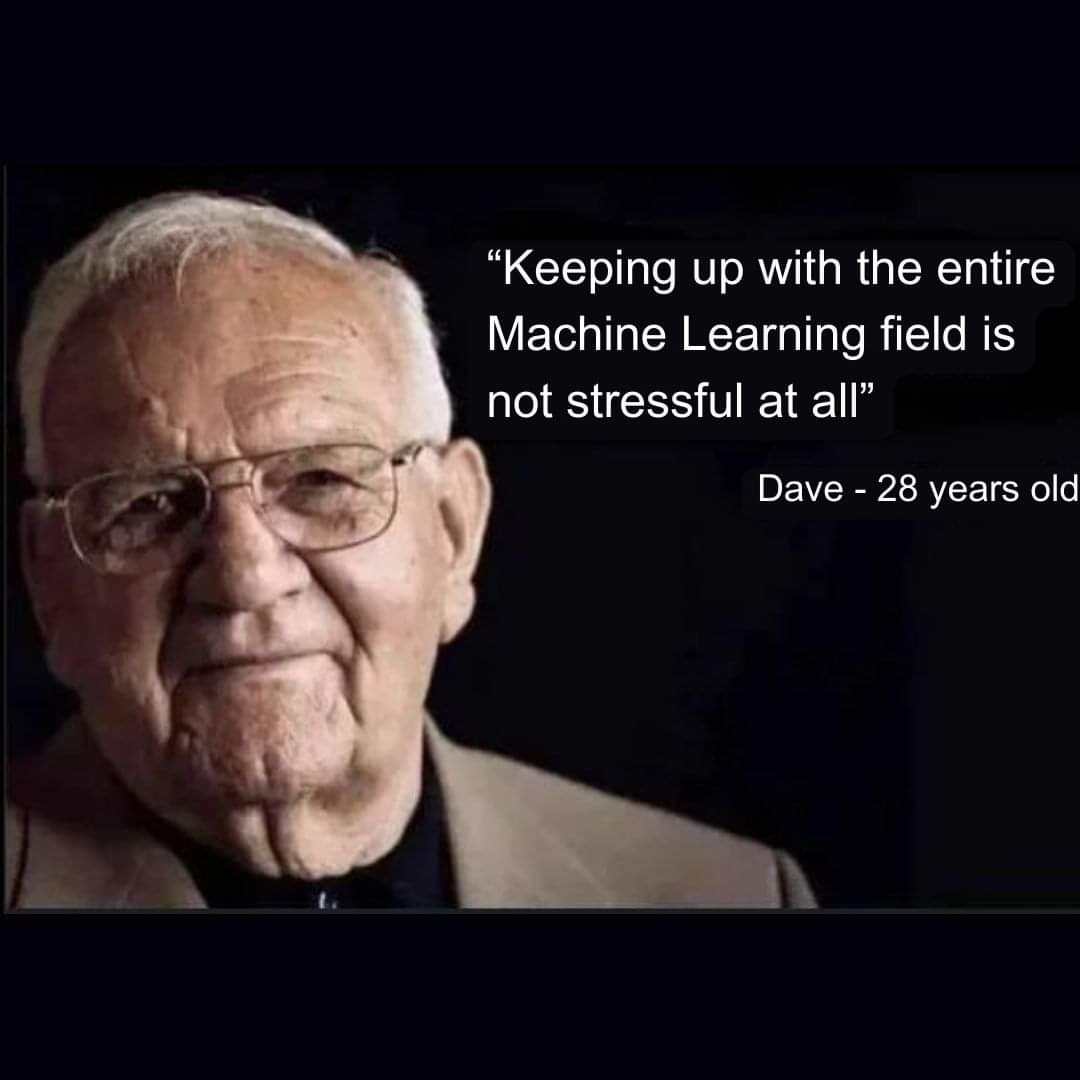
\includegraphics[width=0.7\textwidth,height=\textheight]{content/image/intro/meme_1.jpg}

}

\subcaption{\label{fig-meme1}Learning AI is easy!}

\end{minipage}%
%
\begin{minipage}{0.50\linewidth}

\centering{

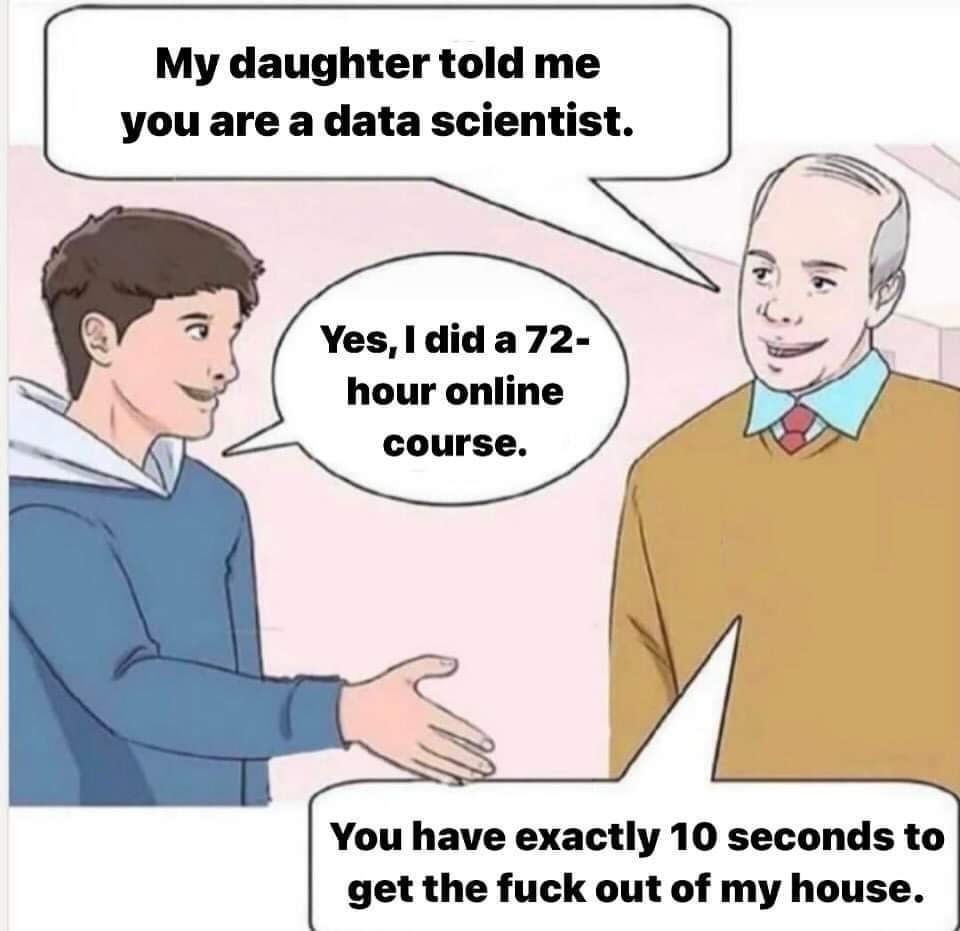
\includegraphics[width=0.7\textwidth,height=\textheight]{content/image/intro/meme_2.jpg}

}

\subcaption{\label{fig-meme2}I am AI expert!}

\end{minipage}%

\caption{\label{fig-meme}Famous Memes}

\end{figure}%

Some notable examples:

\begin{itemize}
\tightlist
\item
  Google (\href{https://arxiv.org/abs/1506.01497v3}{region proposal
  network})
\item
  Google (\href{https://arxiv.org/abs/2205.03983}{Transformer-based})
\end{itemize}

\begin{figure}[H]

\centering{

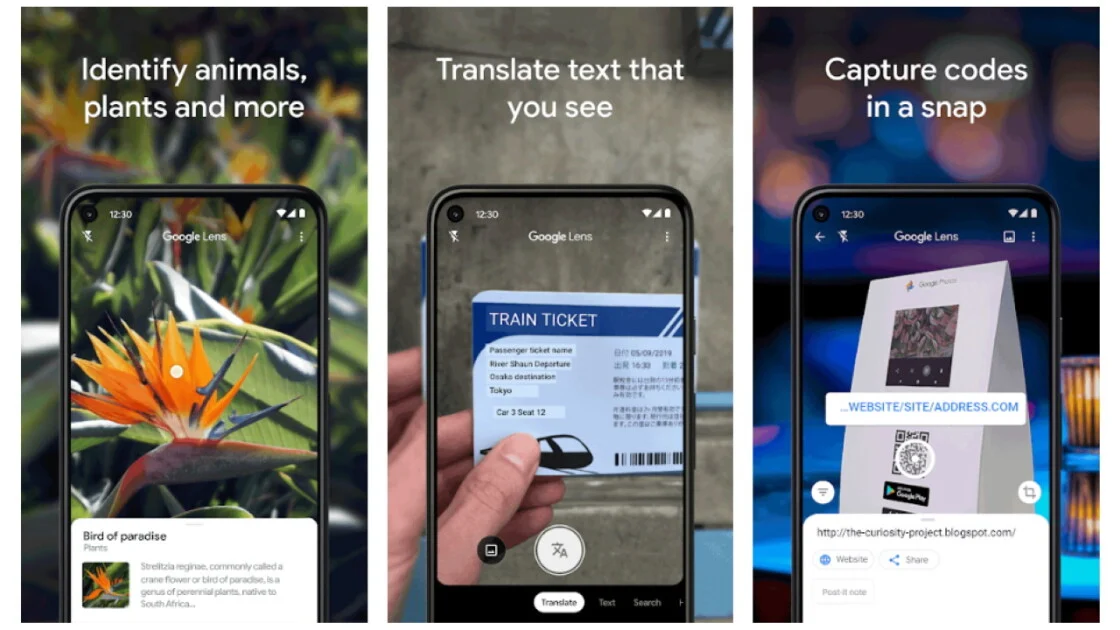
\includegraphics[width=0.7\textwidth,height=\textheight]{content/image/intro/google_lens.png}

}

\caption{\label{fig-ml-google-1}Google Lens \& Translate}

\end{figure}%

\begin{itemize}
\tightlist
\item
  YouTube automatic captioning
  (\href{https://arxiv.org/abs/2005.08100}{automatic speech
  recognition})
\end{itemize}

\begin{figure}[H]

\centering{

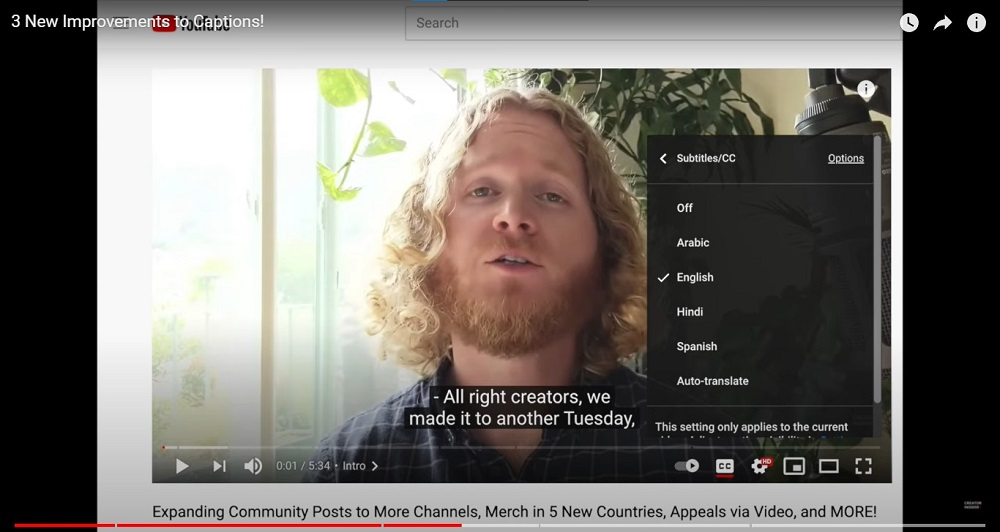
\includegraphics[width=0.7\textwidth,height=\textheight]{content/image/intro/YouTube_Caption_Auto.jpg}

}

\caption{\label{fig-ml-google-2}Google Auto Captioning}

\end{figure}%

\begin{itemize}
\tightlist
\item
  G-mail spam filters (rule-based filters + Density clustering)
\item
  Apple's face-ID
  (\href{https://machinelearning.apple.com/research/face-detection}{deep
  convolutional networks})
\end{itemize}

\begin{figure}[H]

\centering{

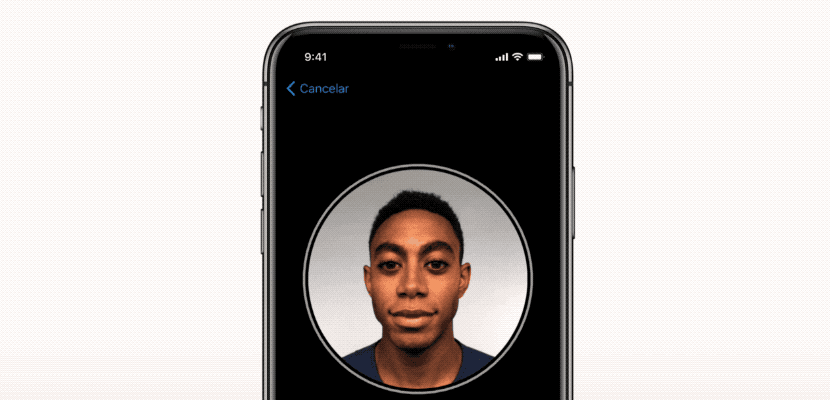
\includegraphics[width=0.7\textwidth,height=\textheight]{content/image/intro/face_ID.png}

}

\caption{\label{fig-ml-faceid}Apple Face-ID}

\end{figure}%

\begin{itemize}
\tightlist
\item
  Tesla autonomous car
  (\href{https://www.youtube.com/watch?v=j0z4FweCy4M}{deep learning})
\end{itemize}

\begin{figure}[H]

\centering{

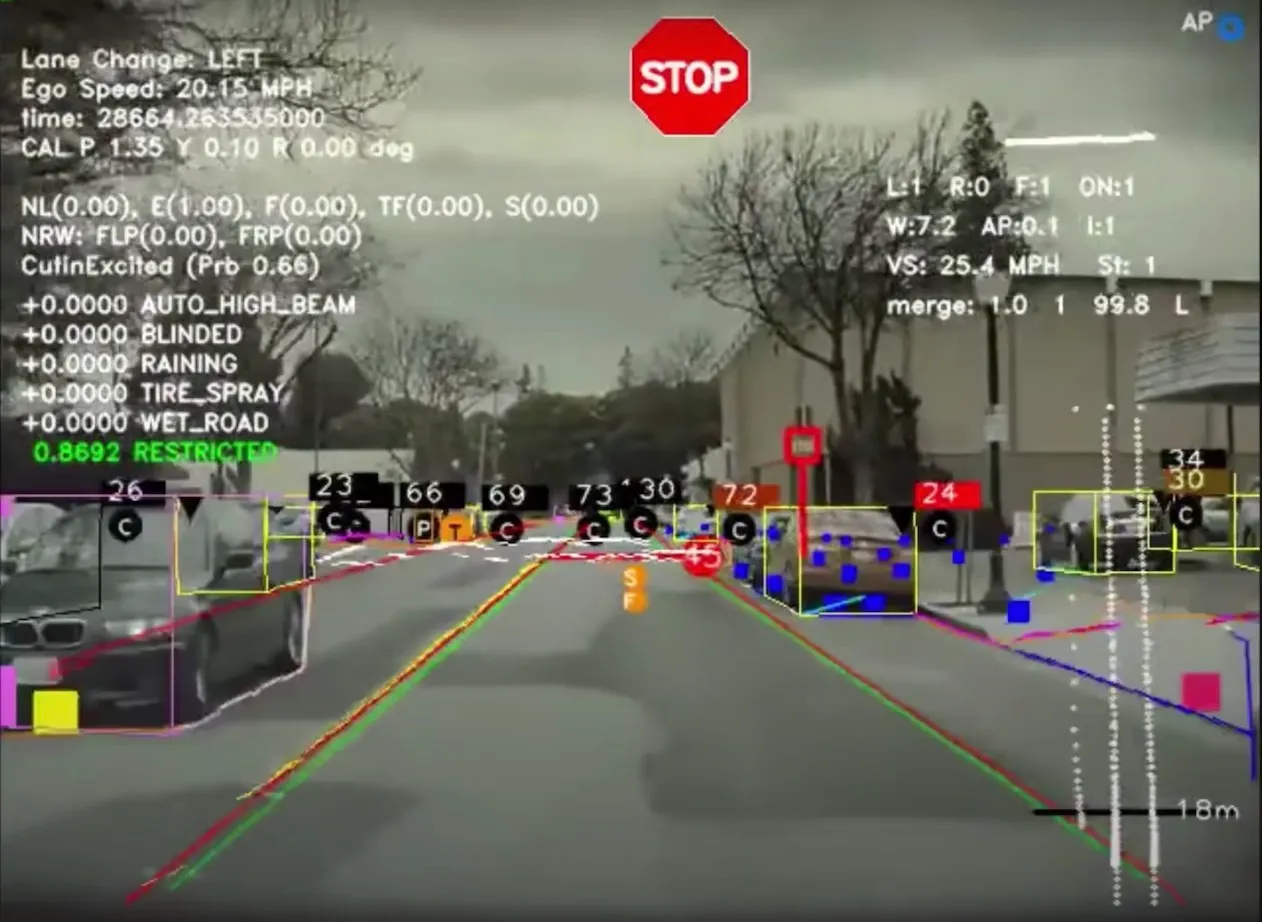
\includegraphics[width=0.7\textwidth,height=\textheight]{content/image/intro/Tesla-object-detection.png}

}

\caption{\label{fig-ml-teslai}Tesla's AI}

\end{figure}%

\begin{itemize}
\tightlist
\item
  virtual assistant (Siri, Google Assistant)
\end{itemize}

\begin{figure}[H]

\begin{minipage}{0.50\linewidth}

\centering{

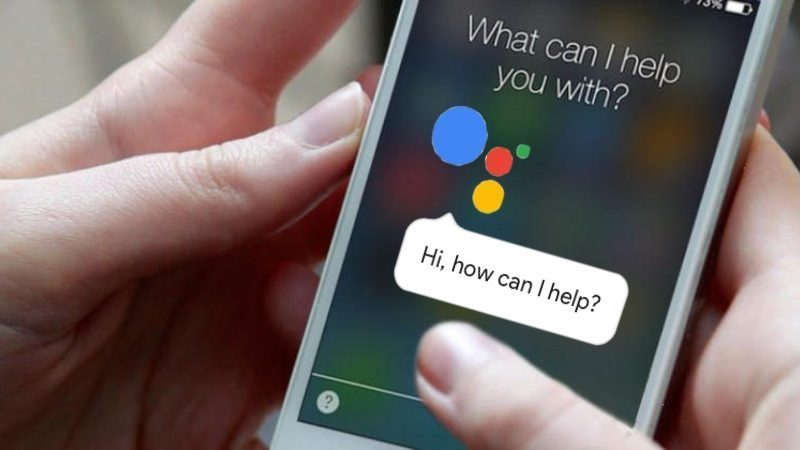
\includegraphics[width=0.7\textwidth,height=\textheight]{content/image/intro/google-assistant.jpg}

}

\subcaption{\label{fig-assist-1}Google Assistant}

\end{minipage}%
%
\begin{minipage}{0.50\linewidth}

\centering{

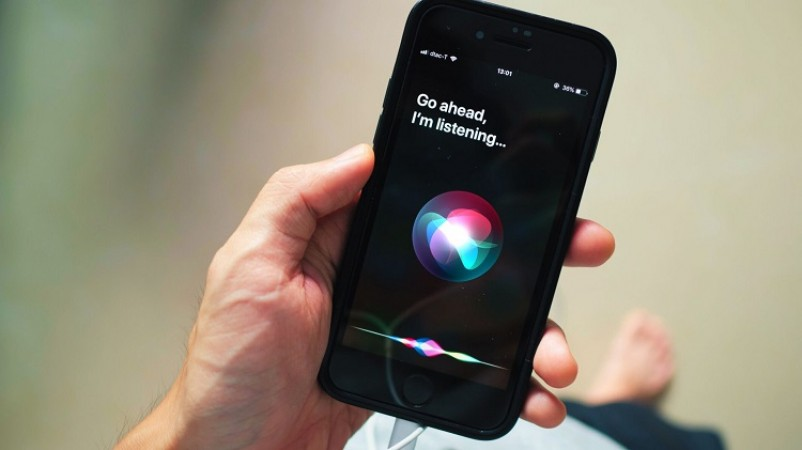
\includegraphics[width=0.7\textwidth,height=\textheight]{content/image/intro/siri-assistant.jpg}

}

\subcaption{\label{fig-assist-2}Apple Siri}

\end{minipage}%

\caption{\label{fig-assistant}Intelligence Chatbot Asssistant}

\end{figure}%

\begin{itemize}
\tightlist
\item
  NVIDIA DLSS
  (\href{https://www.nvidia.com/en-my/geforce/technologies/dlss/}{Deep
  learning supersampling})
\end{itemize}

\begin{figure}[H]

\centering{

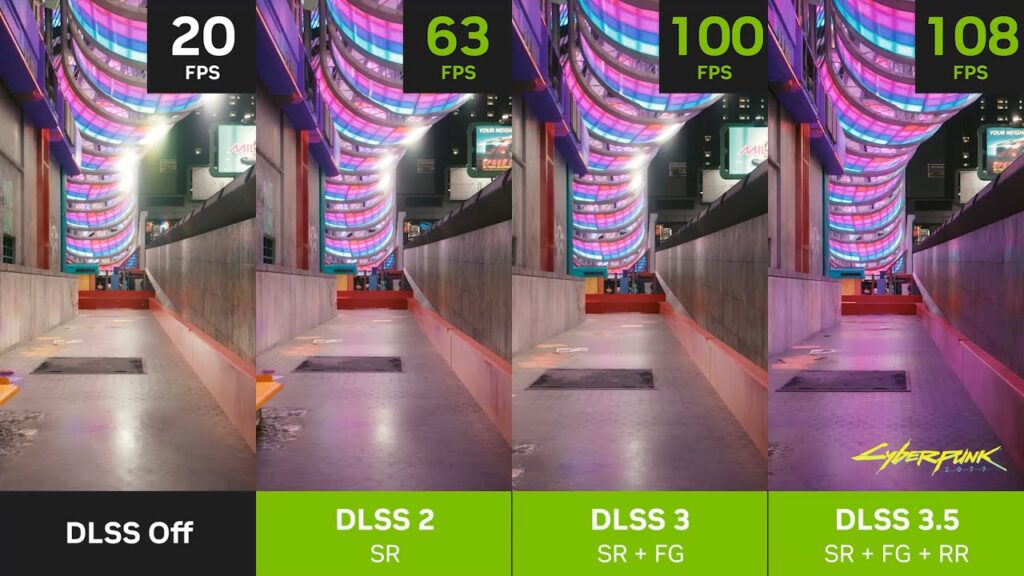
\includegraphics[width=0.7\textwidth,height=\textheight]{content/image/intro/nvidia-dlss.jpg}

}

\caption{\label{fig-nvidia-dlss}NVIDIA DLSS}

\end{figure}%

\begin{itemize}
\tightlist
\item
  Bloomberg
  (\href{https://www.bloomberg.com/company/values/tech-at-bloomberg/artificial-intelligence-ai/}{NLP})
\end{itemize}

\begin{figure}[H]

\centering{

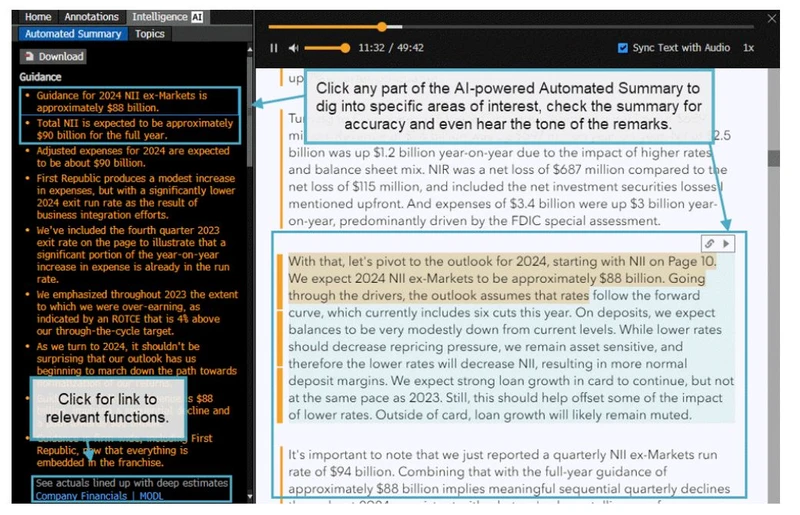
\includegraphics[width=0.7\textwidth,height=\textheight]{content/image/intro/bloomberg_nlp.png}

}

\caption{\label{fig-bloomberg-ai}Bloomberg NLP}

\end{figure}%

Some notable examples (science):

\begin{itemize}
\tightlist
\item
  \href{https://physics.aps.org/articles/v15/74}{Milky Way's Black Hole}
\end{itemize}

\begin{figure}[H]

\centering{

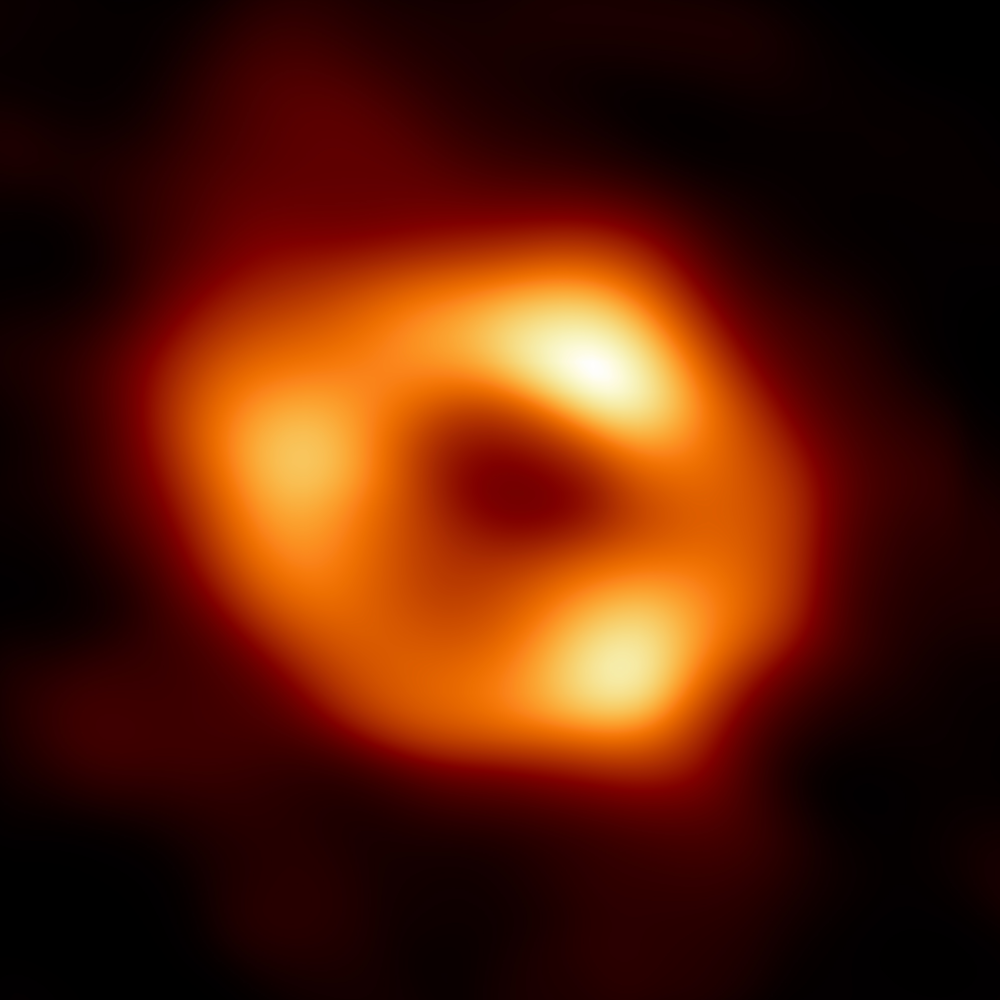
\includegraphics[width=0.4\textwidth,height=\textheight]{content/image/intro/blackhole.png}

}

\caption{\label{fig-BH}First Image of the Milky Way's Black Hole}

\end{figure}%

\begin{itemize}
\tightlist
\item
  \href{https://www.microsoft.com/en-us/research/blog/fs-mol-bringing-deep-learning-to-early-stage-drug-discovery/}{Molecular
  Design}
\end{itemize}

\begin{figure}[H]

\centering{

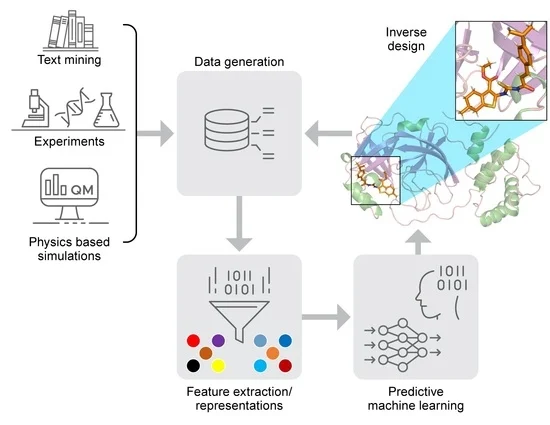
\includegraphics[width=0.4\textwidth,height=\textheight]{content/image/intro/drug-desgn.png}

}

\caption{\label{fig-drug}Drug Discovery}

\end{figure}%

my encounter:

\begin{itemize}
\tightlist
\item
  geospatial intelligence: land use analysis
\end{itemize}

\begin{figure}[H]

\centering{

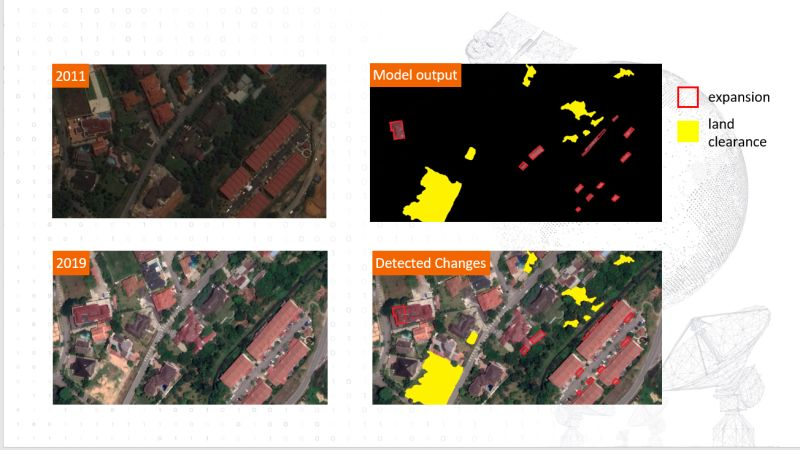
\includegraphics[width=0.7\textwidth,height=\textheight]{content/image/intro/geospatial.jpeg}

}

\caption{\label{fig-geo}Land Clearing Detection (Urban Planning)}

\end{figure}%

\begin{itemize}
\tightlist
\item
  oil \& gas: corrosion detection in confined space
\end{itemize}

\begin{figure}[H]

\centering{

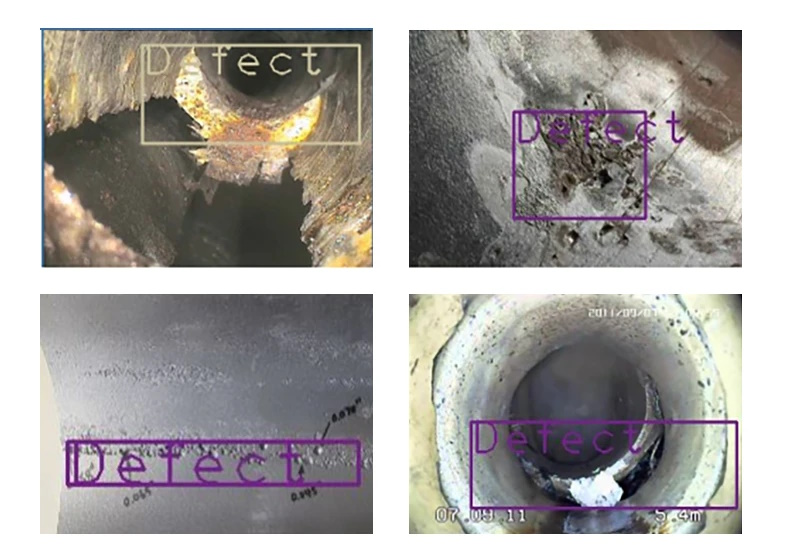
\includegraphics[width=0.7\textwidth,height=\textheight]{content/image/intro/corrosion_detection.jpg}

}

\caption{\label{fig-karat}corrosion detection in pipeline}

\end{figure}%

\begin{itemize}
\item
  automation: vehicle QC inspection (detect scratch, dent on body
  surface)
\item
  automation: vehicle QC inspection (detect missing screw in motorcycle
  assembly line)
\item
  safety: Personal protective equipment (PPE) detection for safety
  inspection
\end{itemize}

\begin{figure}[H]

\centering{

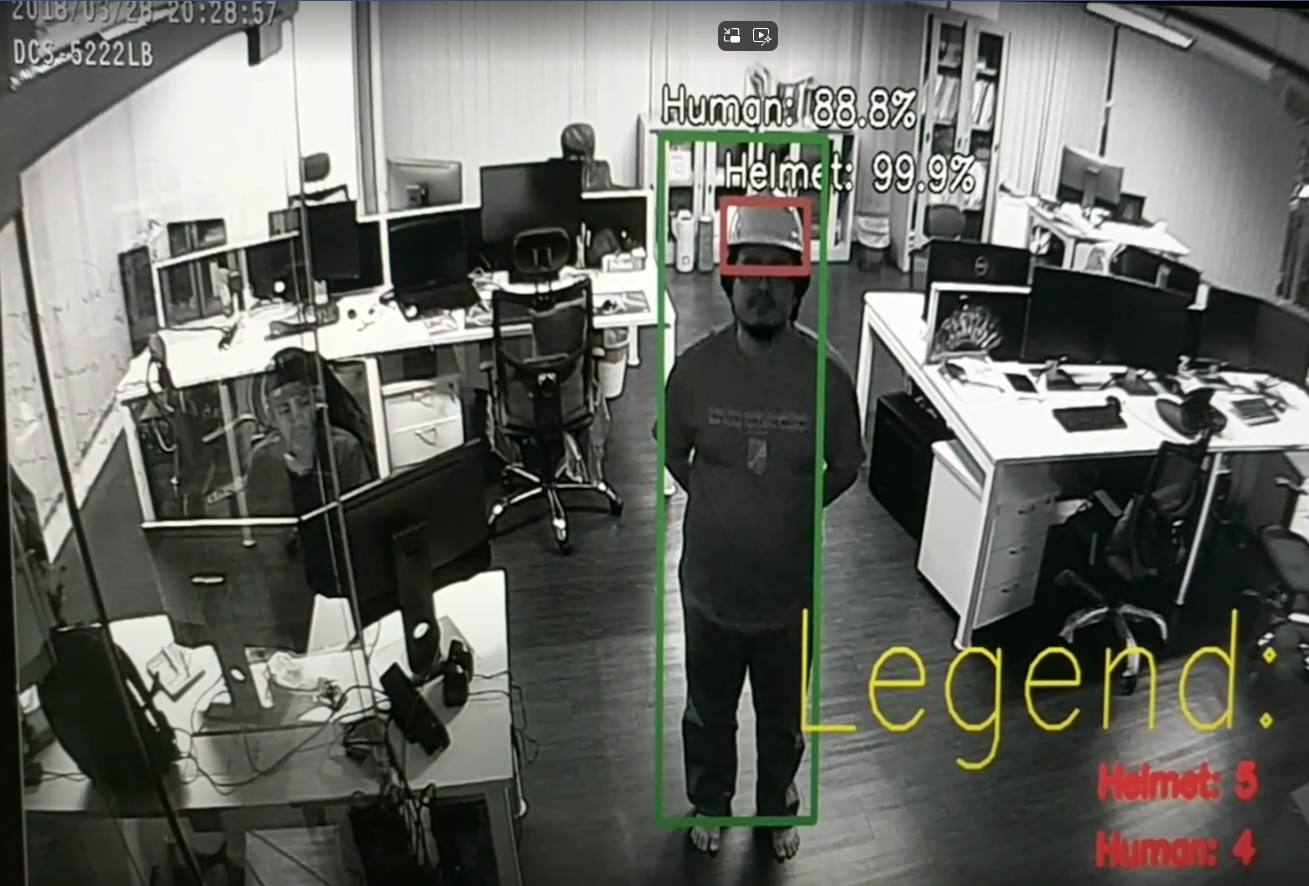
\includegraphics[width=0.4\textwidth,height=\textheight]{content/image/intro/ppe.png}

}

\caption{\label{fig-karat}ppe detection}

\end{figure}%

\begin{itemize}
\tightlist
\item
  finding oil: salt detection
\end{itemize}

\begin{figure}[H]

\centering{

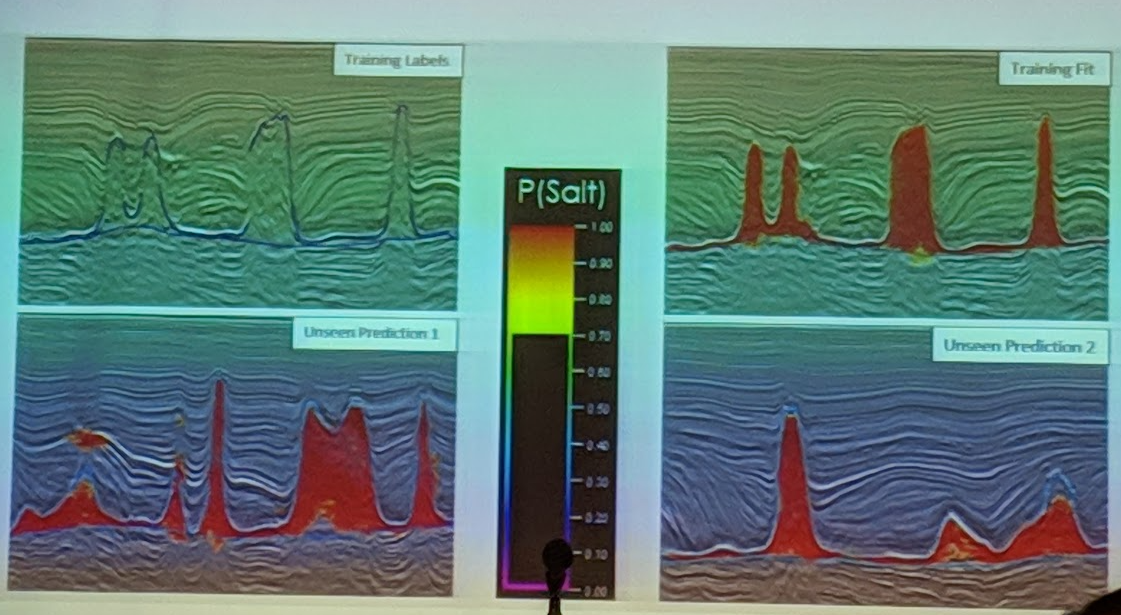
\includegraphics[width=0.6\textwidth,height=\textheight]{content/image/intro/salt_detection.png}

}

\caption{\label{fig-salt}salt detection}

\end{figure}%

\begin{tcolorbox}[enhanced jigsaw, colbacktitle=quarto-callout-caution-color!10!white, arc=.35mm, opacitybacktitle=0.6, titlerule=0mm, opacityback=0, bottomtitle=1mm, title=\textcolor{quarto-callout-caution-color}{\faFire}\hspace{0.5em}{So, why do we need AI?}, breakable, toptitle=1mm, colback=white, rightrule=.15mm, colframe=quarto-callout-caution-color-frame, left=2mm, bottomrule=.15mm, toprule=.15mm, leftrule=.75mm, coltitle=black]

\begin{figure}[H]

\centering{

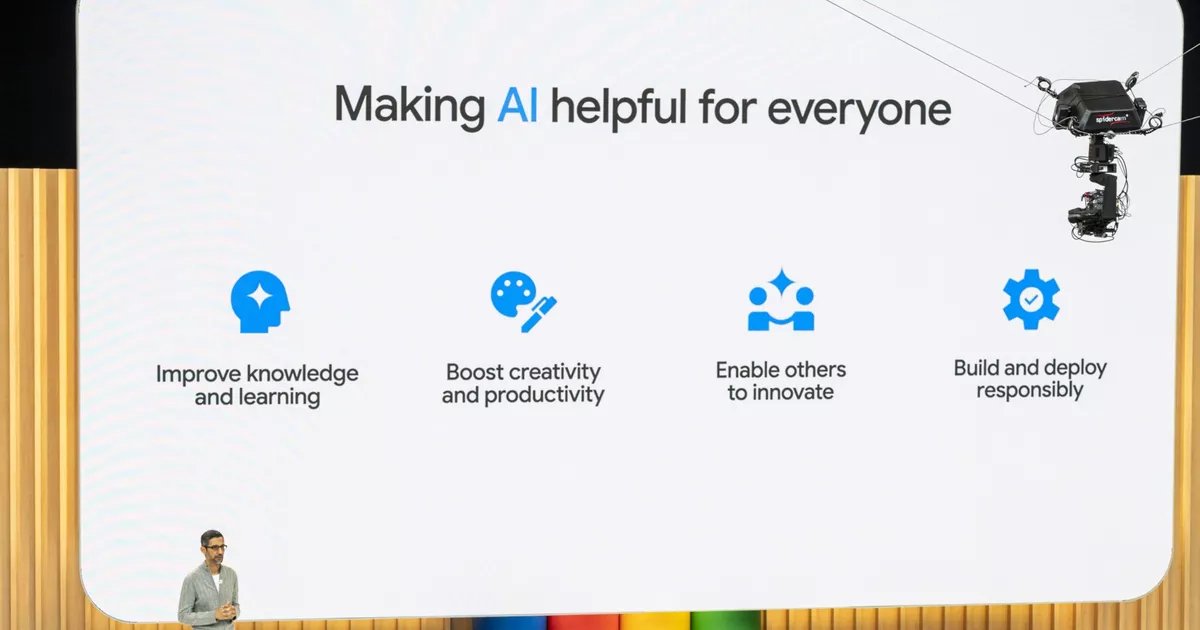
\includegraphics[width=0.7\textwidth,height=\textheight]{content/image/intro/useful.png}

}

\caption{\label{fig-ml-google}General goal of AI\textsuperscript{1}}

\end{figure}%

\end{tcolorbox}

\section{Artificial intelligence, Machine learning and Deep
learning}\label{artificial-intelligence-machine-learning-and-deep-learning}

Data science and statistics - are two of the same, except that in
earlier days, Data Science as we know it today, was called ``statistical
data analysis'' or ``applied statistics''.

``Data Scientist'' means a professional who uses scientific methods to
liberate and create meaning from raw data.

``Statistics'' means the practice or science of collecting and analyzing
numerical data in large quantities.

There are no real difference between the two, except that ``Data
Scientists'' prowes in large scale data or Big Data and fast computing.
Otherwise, they are the same.

Today, there are no difference between the two.\textsuperscript{2}

\begin{figure}[H]

\centering{

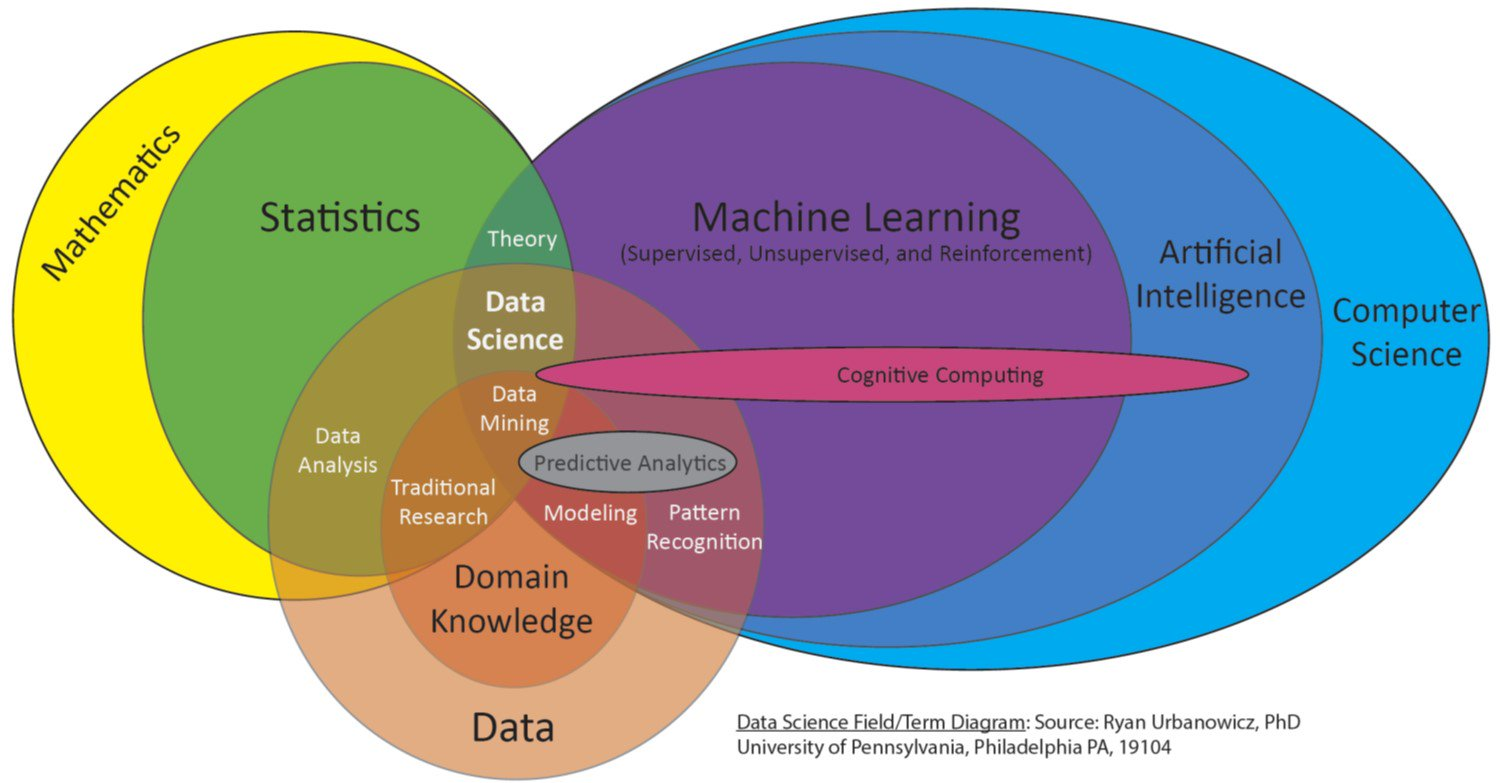
\includegraphics[width=0.7\textwidth,height=\textheight]{content/image/intro/venn_diagram.jpeg}

}

\caption{\label{fig-semua}Everything everywhere all at
once\textsuperscript{3}}

\end{figure}%

\begin{figure}[H]

\centering{

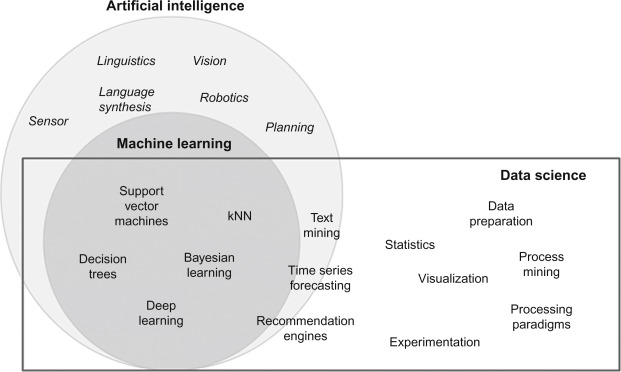
\includegraphics[width=0.7\textwidth,height=\textheight]{content/image/intro/relationship.jpg}

}

\caption{\label{fig-ml-kaitan}Artificial intelligence, machine learning,
and data science.\textsuperscript{4}}

\end{figure}%

The central goal of AI is to provide a set of algorithms and techniques
that can be used to solve problems that humans perform
\emph{intuitively} and near \emph{automatically}. A great example of
such a class of AI problems is interpreting and understanding the
contents of an image -- this task is something that a human can do with
little-to-no effort, but it has proven to be extremely difficult for
machines to accomplish.

\begin{tcolorbox}[enhanced jigsaw, colbacktitle=quarto-callout-tip-color!10!white, arc=.35mm, opacitybacktitle=0.6, titlerule=0mm, opacityback=0, bottomtitle=1mm, title=\textcolor{quarto-callout-tip-color}{\faLightbulb}\hspace{0.5em}{How do we relate it all?}, breakable, toptitle=1mm, colback=white, rightrule=.15mm, colframe=quarto-callout-tip-color-frame, left=2mm, bottomrule=.15mm, toprule=.15mm, leftrule=.75mm, coltitle=black]

Deep learning is a subfield of machine learning, which is, in turn, a
subfield of artificial intelligence (AI).

\end{tcolorbox}

Machine learning tends to be specifically interested in
\textbf{\emph{pattern recognition}} and \textbf{\emph{learning from
data}}. Artificial Neural Networks (ANNs) are a class of machine
learning algorithms that learn from data and specialize in pattern
recognition, inspired by the structure and function of the brain.

Deep learning is an approach to AI. It is a type of machine learning, a
technique that allows computer systems to improve with experience and
data.

\section{Data Scientist vs Machine Learning
Engineer}\label{data-scientist-vs-machine-learning-engineer}

\begin{figure}[H]

\centering{

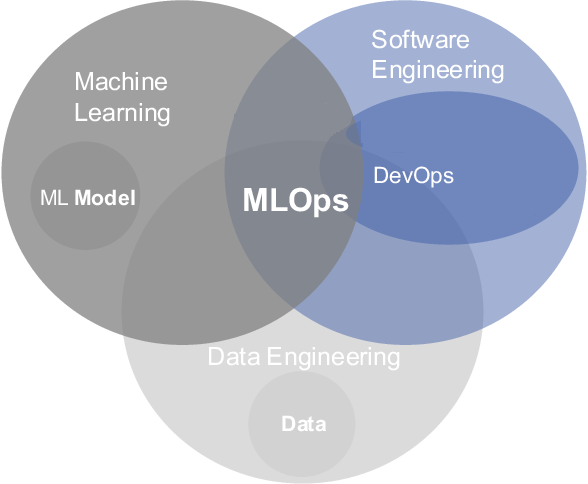
\includegraphics[width=0.7\textwidth,height=\textheight]{content/image/intro/ml_ops.png}

}

\caption{\label{fig-ml-kaitan}Domain area of deep
learning\textsuperscript{5}}

\end{figure}%

MLOps is the process of automating and \emph{\textbf{productize}}
machine learning applications and workflows.

\section{Reality: ML in production}\label{reality-ml-in-production}

Machine learning in production is very complicated!

\begin{figure}[H]

\centering{

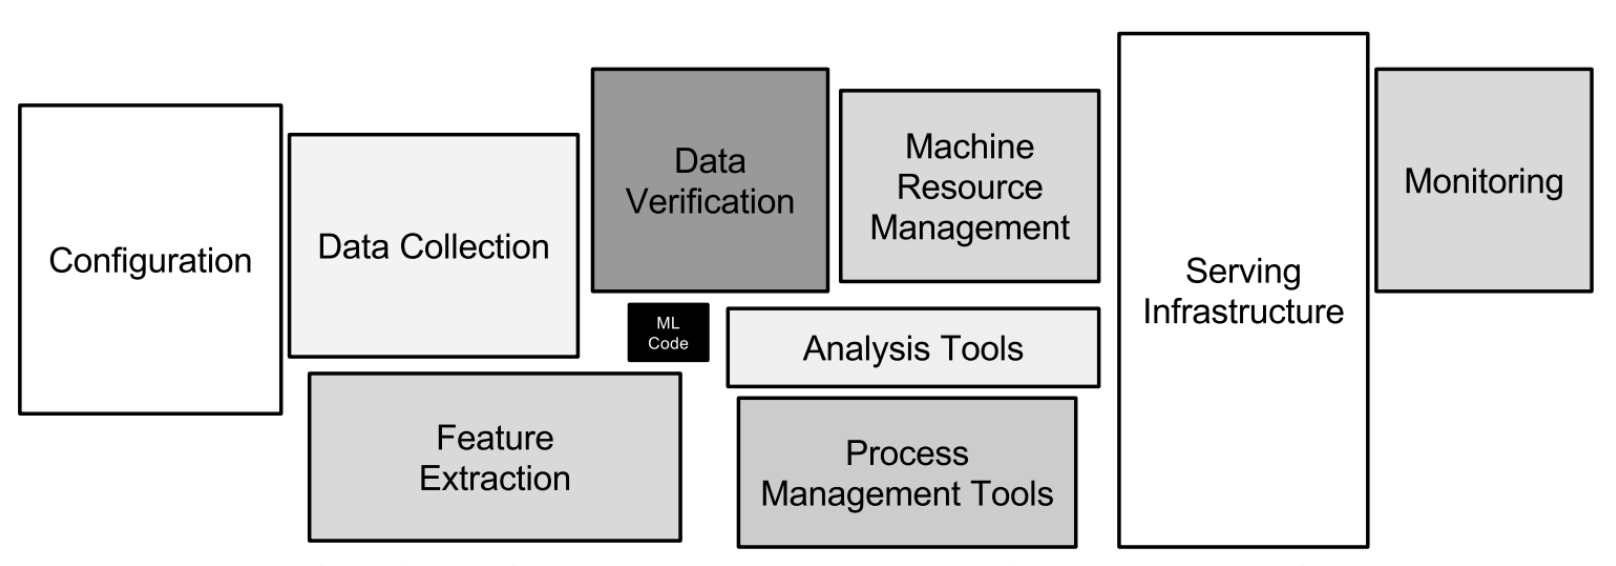
\includegraphics[width=0.7\textwidth,height=\textheight]{content/image/intro/technical_debt.png}

}

\caption{\label{fig-ml-kaitan}Only a small fraction of real-world ML
systems is composed of the ML code, as shown by the small black box in
the middle. The required surrounding infrastructure is vast and
complex.\textsuperscript{6}}

\end{figure}%

In a perfect world, data scientist will do ML modelling while ML
Engineer will productize ML model from Data Scientist. In reality
(especially in Small \& Medium Enterprise), Data Scientist \& ML
Engineer job scope is intertwine (or even the same person!)

\begin{figure}[H]

\centering{

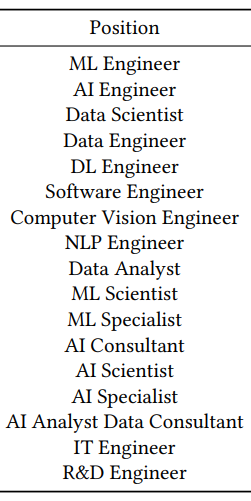
\includegraphics[width=0.2\textwidth,height=\textheight]{content/image/intro/work_list.png}

}

\caption{\label{fig-work-list}Categories of job titles related to AI}

\end{figure}%

\begin{figure}[H]

\centering{


\includegraphics[width=0.4\textwidth,height=\textheight]{content/image/intro/gaji.jpeg}

}

\caption{\label{fig-meme3-gaji}Is this true?}

\end{figure}%

So, knowing Figure~\ref{fig-work-list}, is Figure~\ref{fig-meme3-gaji}
true? From Figure~\ref{fig-work-list}, AI Scientist/Researcher have a
place in Malaysian Market?

\begin{tcolorbox}[enhanced jigsaw, colbacktitle=quarto-callout-important-color!10!white, arc=.35mm, opacitybacktitle=0.6, titlerule=0mm, opacityback=0, bottomtitle=1mm, title=\textcolor{quarto-callout-important-color}{\faExclamation}\hspace{0.5em}{Exercises}, breakable, toptitle=1mm, colback=white, rightrule=.15mm, colframe=quarto-callout-important-color-frame, left=2mm, bottomrule=.15mm, toprule=.15mm, leftrule=.75mm, coltitle=black]

\begin{itemize}
\tightlist
\item
  Formulate your own definition of artificial intelligence.
\item
  How do we test this intelligence empirically (testable and verifiable
  by observation)?
\item
  We are nowhere near human-level AI today. What are we missing?
\item
  Is AI a science, or is it engineering? Or neither or both? Explain.
\item
  Extra: Does thinking and reasoning require language to work?
\end{itemize}

\end{tcolorbox}

\phantomsection\label{refs}
\begin{CSLReferences}{0}{0}
\bibitem[\citeproctext]{ref-Gugel}
\CSLLeftMargin{1. }%
\CSLRightInline{Google.
\href{https://www.youtube.com/watch?v=QpBTM0GO6xI&list=TLGGCy91ScdjTPYwNTEyMjAyMw}{Google
i/o 2023}. (2023).}

\bibitem[\citeproctext]{ref-Donoho}
\CSLLeftMargin{2. }%
\CSLRightInline{Donoho, D.
\href{https://doi.org/10.1080/10618600.2017.1384734}{50 years of data
science}. \emph{Journal of Computational and Graphical Statistics}
\textbf{26}, 745--766 (2017).}

\bibitem[\citeproctext]{ref-Ryan}
\CSLLeftMargin{3. }%
\CSLRightInline{Urbanowicz, R.
\href{https://twitter.com/DocUrbs/status/1007375834347376642?lang=en}{Proposed
field/term venn diagram}. (2018).}

\bibitem[\citeproctext]{ref-KOTU20191}
\CSLLeftMargin{4. }%
\CSLRightInline{Kotu, V. \& Deshpande, B.
\href{https://www.sciencedirect.com/science/article/pii/B9780128147610000010}{Chapter
1 - introduction}. in \emph{Data science (second edition)} (eds. Kotu,
V. \& Deshpande, B.) (Morgan Kaufmann, 2019).}

\bibitem[\citeproctext]{ref-Prabhu}
\CSLLeftMargin{5. }%
\CSLRightInline{Prabhu.
\href{https://medium.com/aimonks/the-rise-of-mlops-managing-machine-learning-at-scale-e31ea4a0039f}{The
rise of MLOps: Managing machine learning at scale}. (2023).}

\bibitem[\citeproctext]{ref-NIPS2015_86df7dcf}
\CSLLeftMargin{6. }%
\CSLRightInline{Sculley, D. \emph{et al.}
\href{https://proceedings.neurips.cc/paper_files/paper/2015/file/86df7dcfd896fcaf2674f757a2463eba-Paper.pdf}{Hidden
technical debt in machine learning systems}. in \emph{Advances in neural
information processing systems} (eds. Cortes, C., Lawrence, N., Lee, D.,
Sugiyama, M. \& Garnett, R.) vol. 28 (Curran Associates, Inc., 2015).}

\end{CSLReferences}


\backmatter

\end{document}
